%=========================================================
% Floating Point CSR
%=========================================================
\section{Floating Point CSR}

The Floating Point Unit of mmRISC-1 uses Goldschmidt's Algorithm for FDIV.S and FSQRT.S instructions. A CSR FCONV, which is a dedicated CSR of mmRISC-1, configures the convergence loop count for each FDIV and FSQRT. The larger loop counts generate more precise results.

\begin{table}[H]
    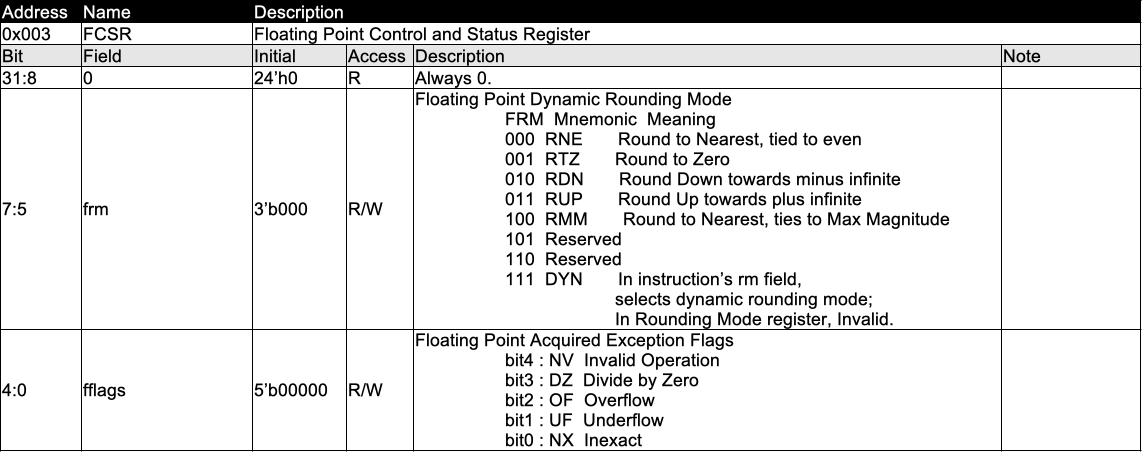
\includegraphics[width=1.00\columnwidth]{./Table/FCSR.png}
    \caption{FCSR}
    \label{tb:FCSR}
\end{table}

\begin{table}[H]
    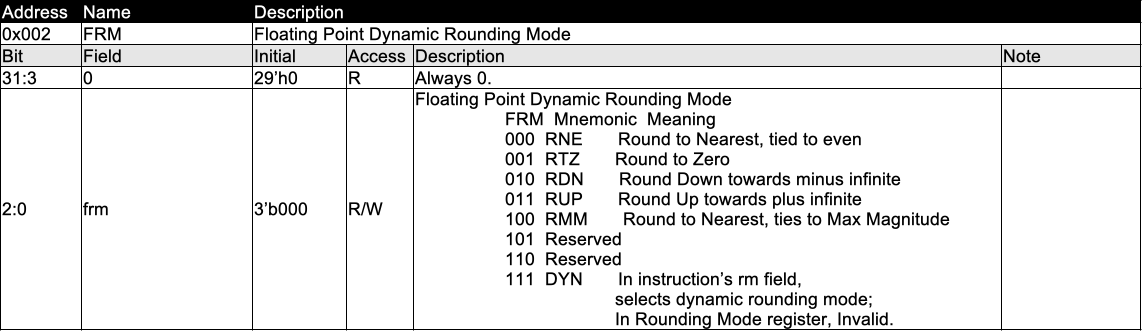
\includegraphics[width=1.00\columnwidth]{./Table/FRM.png}
    \caption{FRM}
    \label{tb:FRM}
\end{table}

\begin{table}[H]
    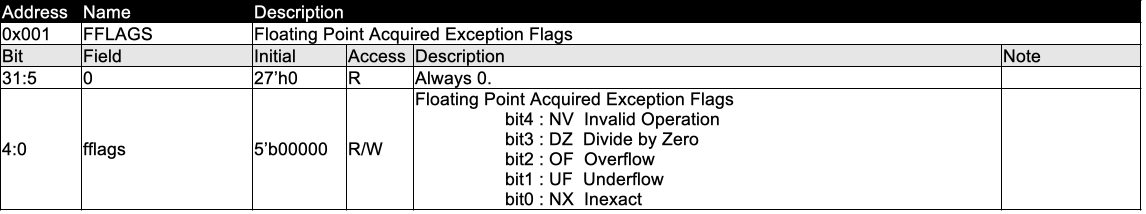
\includegraphics[width=1.00\columnwidth]{./Table/FFLAGS.png}
    \caption{FFLAGS}
    \label{tb:FFLAGS}
\end{table}

\begin{table}[H]
    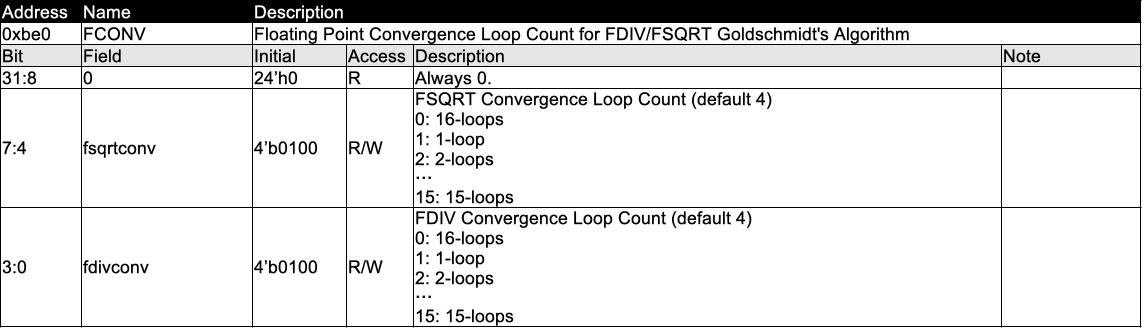
\includegraphics[width=1.00\columnwidth]{./Table/FCONV.png}
    \caption{FCONV}
    \label{tb:FCONV}
\end{table}

